\documentclass[12pt,a4paper,titlepage]{article}
\usepackage[utf8]{inputenc}
\usepackage{amsmath}
\usepackage{amsfonts}
\usepackage{amssymb}
\usepackage{supertabular}
\usepackage{tabularx}
\usepackage{ltablex}
\usepackage{graphicx}
\usepackage{pdfpages}
\usepackage[left=1in,right=1in,top=1in,bottom=1in]{geometry}
\parskip=12pt
\setlength{\parindent}{0pt}
% sorry Keith, but I like this paragraph style better...
\title{
		\center\textbf{\Large{Metrics Report}\\
		\large{Including Analysis of Coverage, Complexity, Cohesion, and Coupling\\
		For\\
		\large{Swords and Sorcery(S\&S)}}\\
		Version 1.0}}
\author{Prepared by:\\University of Idaho Computer Science 383 Class, Spring 2014\\
\bigskip\\
Prepared for:\\
Dr. Clinton Jeffery\\} 
\date{\today} 
\begin{document}
\maketitle
\pagebreak
\setcounter{tocdepth}{3}
\renewcommand\contentsname{\center{Swords and Sorcery Metrics\\Table of Contents}}
\tableofcontents
\pagebreak

\section{Introduction}
This document includes reports and analysis of several software metrics of our computer 
adaptation of the Swords \& Sorcery board game. The project and its documentation are 
property of the Spring 2014 Software Engineering class at the University of Idaho 
and its constituents.

Through this document, the development team aims to describe the software using several 
measurements such as Test Coverage, Complexity, Coupling, and Cohesion. Analysis of these 
metrics and what they mean for the software follow.

\section{Test Coverage}
The project's 79 automated test cases resulted in 9\% instruction coverage and 5\% branch 
coverage of the entire project. While the average is low for the whole project, some 
elements exhibit higher levels of coverage.

The leader in instruction coverage was the MoveCalculator package, which experienced 
53\% instruction coverage (and 44\% branch coverage). Meanwhile, the most branch coverage 
was attained by the ssterrain package, at 53\% (and 48\% of instructions).

The top level coverage data is summarized by the table below.

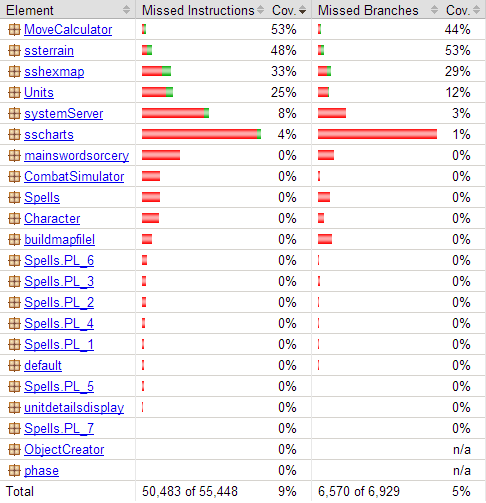
\includegraphics{top_level_coverage}

Ignoring percentages, the package with the most covered instructions was ssterrain with 
1,374 covered instructions. Of its 39 classes, only 10 were missed by the automated 
unit tests. All hex edge types had 100\% coverage except for HEFord. While the various 
terrain types were not covered well, TerrainType itself had 94\% instruction coverage.

You'll notice from the table that the sscharts package sticks out sorely as far as coverage 
goes. This is due largely to the very large and completely untested class CreatUnits, which 
has 14,363 instructions. This is demonstrated below.

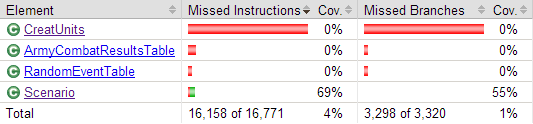
\includegraphics{sscharts_coverage}

Whilte sscharts gets a bad report due to one untested monster, the systemServer package 
warrants its bad marks by leaving several significant classes untested, as shown by the 
following.

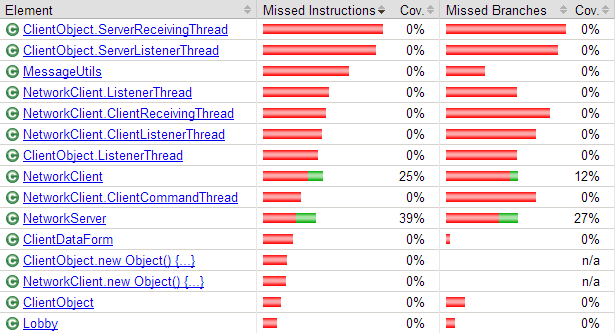
\includegraphics{systemServer_coverage}

The full coverage report can be accessed in the sworsorc repository as sworsorc/.jacocoverage/report.html/index.html for full details.

sshexmap has 16 classes and 9 were missed.  The best coverage was with the Hex class with 
100\% coverage, followed by HexMap with 78\% and MapHex with 69\%. Of the 140 methods in all 
the sshexmap classes 97 were missed and the 801 lines, 550 were missed.

Units has 291 classes and 234 were missed.  The classes that had 100\% coverage were Zeppelin, 
Bow, RangedLandUnit, LandUnit and FlyingUnit.  Of the 156 methods in all the classes of Units 
110 were missed and of the 922 lines 716 were missed.  The UnitPool had 47\% coverage.

Because test coverage in most cases was extremely poor for this project, we have done very 
little to assure that the componenets of the project perform as they are expected to. This 
means that very little can be said about the quality of the product. Our tests simply cannot 
conclude that it performs well. When we analyze the complexity of various components later, 
we will see that some of our worst coverage overlaps with our most complex methods. It 
becomes impossible to assure product quality when the components that are most difficult to 
understand are also unchecked.

\section{Complexity}
When setting out to to develop a semester project for this course, we knew that it would have 
to be complex enough to take a multi-person team of developers a semester to create. These 
complexity metrics serve the dual purpose of assuring the reader that this has occurred while 
also pointing out exactly how frightening it is that test coverage is so low.

\subsection{Lines of Code (LOC)}
The project totals 49,862 lines of code. These are broken up between several packages, with 
the following five having the highest LOC count:

\begin{itemize}
\item src: 40903
\item model: 10485
\item src: 10218
\item CombatSimulater: 10218
\item utilities: 9777
\end{itemize}

The following five classes are the longest as well:

\begin{itemize}
\item Main: 6597
\item CreatUnits: 6575
\item NetworkClient: 1281
\item CharacterJ: 1222
\item CharacterJ: 1222
\end{itemize}

You'll observe that despite breaking the project up into several modules, there are still some 
files that total over six thousand lines of code. This could degrade both the readability 
and maintainability of the code base, as it requires a great deal of effort just to 
understand the code of one class.

\subsection{Class Count}
Even with some classes being so voluminous, we still managed to acquire 303 total classes 
throughout the course of development. Once again, this can have a poor effect on the 
understandability of the project. The packages with the most classes are listed.

\begin{itemize}
\item src: 244
\item model: 119
\item src: 70
\item CombatSimulater: 70
\item doc: 59
\end{itemize}

\subsection{Method Count}
There are a total of 1614 methods. These are more evenly distributed through classes, as shown 
by the top five classes by method count. While this is still a lot of methods for a single 
class to contain, at least there are no outlying monsters in this respect.

\begin{itemize}
\item NetworkClient: 42
\item CharacterJ: 42
\item CharacterJ: 42
\item MainMap: 35
\item MapHex: 30
\end{itemize}

\subsection{McGabe's Cyclomatic Complexity}
While the average cyclomatic complexity of the project's methods was a comfortable 3.33, 
outliers emerge that are purely terrifying. The unchecked CreatUnits class provides one of 
these, while the others are equally unchecked methods within Main.

\begin{itemize}
\item Main::Create\_unit1: 252
\item Main::Create\_unit2: 252
\item Main::Create\_unit4: 252
\item Main::Create\_unit3: 252
\item CreatUnits::Create\_unit2: 202
\end{itemize}

These monstrously-complex methods include nested switch statements (thus the high volume of 
paths possible), and it is unclear what they are meant to do. This has a disastrous effect 
on readability, comprehension, and maintainability. Furthermore, something this complex 
and untested is likely to be broken, meaning that maintainability and quality are also 
affected in that sense.

\section{Coupling}
Our metrics tools gave the following measurements of coupling.

Loose Class Coupling (LCC) averaged 0.151 with a maximum of 1 and a minimum of 0 for the project.
High Class Coupling (HCC) on the other hand also ranged from 0 to 1 and averaged 0.111.

From this data, we can conclude that about 15\% of our classes are loosely coupled, 
meaning they require little knowledge of the definitions provided in other classes. 
This means that these classes may experience an increase in readability, maintainability, 
and testability because they can stand alone.

On the other hand, about 11\% of our classes were tightly coupled, which means understanding, 
testing, and executing them requires knowledge of the definitions in other classes. This can 
be detrimental to maintainability, testability, and readability.

\section{Cohesion}
The five measure sof Lack of Cohesion had the following minimums, maximums, and averages for 
the project.

\begin{enumerate}
\item 32, 299, 43
\item 28, 273, 39
\item 2, 6, 5
\item 2, 6, 4
\item 0.925, 0, 0.553
\end{enumerate}

From these metrics, we can make the following conclusions.

\begin{enumerate}
\item There is a minimum of 32 and at most 299 pairs of methods in a single class that do 
  not share attributes. There is an average of 43 methods per class with low-cohesion.
\item There is a minimum of 28 and at most 273 methods after subtracting the number of pairs of 
  methods that share attributes from the number of pairs of methods that do not share 
  attributes.
\item There is a minimum of 2 and maximum of 6 disjoint components per class with an average 
  of 5 disjoint components per class.
\item Similar to Method3 but measuring method invocations instead of node edges.
\item LCOM5 \= (a – kl) \/ (l – kl), where l is the number of attributes, k is the number of 
  methods, and a is the summation of the number of distinct attributes accessed by each 
  method in a class. The average lack of cohesion across all our classes using LCOM5 is 55.3\%
\end{enumerate}

Unfortunately, some of these measures of Lack of Cohesion are fairly high, meaning we have 
fairly poor cohesion between our classes. Unfortunately, a lack of cohesion can mean that 
the methods and data in classes are unrelated. This has the effect of reducing readability and 
maintainability of methods. Additionally, since classes with unrelated elements are likely to 
be constructed in a design-specific manner that will limit their reusability.

\section{Appendix}
A report of several more metrics can be found as generated by the NetBeans Source Code Metrics 
plugin at sworsorc/doc/EndingDocumentation/Metrics/metrics.xlsx.

\end{document}
